\providecommand{\main}{../../../..}
\documentclass[\main/dresen_thesis.tex]{subfiles}

\begin{document}
  \paragraphNewLine{Scanning Electron Microscopy}
    The spin-coated nanospheres on silicon substrate are qualitatively viewed by SEM micrographs measured with a Neon Zeiss 40 (\refsec{ch:instruments:laboratoryInstruments:sem}).
    To obtain cross-sectional views, a piece of a sample is cut on two opposing sides with a diamond cutter and then subsequently broken downward to obtain a clean breaking line, from which SEM measurements can be performed.
    The micrographs are measured at $5 \unit{kV}$ and the images from the backscattering electrons are shown to obtain a strong contrast.

  \paragraphNewLine{Grazing-Incidence Small-Angle X-ray Scattering}
    All spin-coated samples were measured at the beam line BM26B \refsec{ch:lss:BM26B} in the ESRF at a wavelength of $\lambda \eq 1.03 \unit{\angstrom}$.
    For each sample a measurement was performed at a large sample-to-detector distance of $6.54 \unit{m}$ and at a shorter sample-to-detector distance of $2.90 \unit{m}$.
    The collimation slit is set to $0.3 \times 0.5 \unit{mm^2}$ for each measurement, and every sample is evaluated at an incident angle of $0.2 \unit{^\circ}$.

    For both samples, a strip of $0.02 \nm^{-1}$ width along the Yoneda band is integrated and compared to the form factor obtained by small-angle X-ray scattering.
    The scattered intensity for the nanostructure along the Yoneda band is calculated as product of a structure factor and the form factor
    \begin{align}
      I(q) \eq I_0 S(q) |P(q)|^2 + I_\mathrm{bg},
    \end{align}
    where $I_0$ is a scaling factor and $I_\mathrm{bg}$ is a incoherent noise background that is not directly associated with the scattering from the nanoparticles.
    The used form factor $|P(q)|^2$ is hereby given by using the best fit of the nanoparticles from SAXS as determined in \refsec{sec:looselyPackedNS:nanoparticle:sas}.
    As no calibration measurement has been performed at BM26B, the data is given in the arbitrary count units of the detector.
    The structure factor for hard spheres of radius $R_\mathrm{HS}$ and with a packing fraction $\eta$ can be calculated analytically in the Percus-Yervick approximation \cite{Percus_1958_Analy, Wertheim_1963_Exact, Pedersen_1997_Analy} and is given by
    \begin{align}
      S(q) &\eq \frac{1}{1 + 24 \eta \frac{G(2 q R_\mathrm{HS})}{2 q R_\mathrm{HS}} }
    \end{align}
    with
    \begin{align}
      \begin{split}
        G(x)   &\eq \frac{(1 + 2\eta )^2}{(1 - \eta )^4} \cdot \frac{ \sin(x) - x \cos(x)}{x^2}\\
               & + \frac {-6 \eta (1 + \eta / 2)^2}{(1 - \eta )^4} \cdot \frac{2 x sin(x) + (2 - x^2) \cos(x) - 2}{x^3}\\
               & + \frac{\eta (1 + 2\eta )^2}{2(1 - \eta )^4} \cdot \frac{-x^4 \cos(x) + 4 [(3 x^2 - 6) \cos(x) +(x^3 - 6 x) \sin(x) + 6]}{x^5}\\
      \end{split}
    \end{align}

  \paragraphNewLine{X-Ray Reflectometry}
    XRR was performed using a Bruker D8 Advanced at the \textsc{Forschungszentrum J\"ulich} \refsec{ch:instruments:laboratoryInstruments:xrr}.
    The X-ray reflectometer was equipped with a Cu-K$\alpha$ source ($\lambda \eq 1.54 \unit{\angstrom}$) and a $q$-range of $0 \ldots 0.15 \unit{\angstrom^{-1}}$ is evaluated by measuring $2 \theta \eq 0 \ldots 1 \unit{^\circ}$ in $0.005 \unit{^\circ}$ steps over an integrated time of approximately $1 \unit{h}$.
    The collimation slit on the instrument is $0.2 \unit{mm}$ and both samples have a width of approximately $20 \unit{mm}$.

    To evaluate the reflectivity, a footprint correction is performed as described in \refsec{ch:methods:xrr}, assuming a equidistributed beam profile.
    As substrate, the scattering length density of silicon is fixed to the literature value at the given wavelength ($\rho_\mathrm{Si} \eq 20.062 \cdot \unit{10^{-5} \angstrom^{-2}}$) and a spacer layer is allowed for the case of a thin \ch{SiO2} or any organic residues in between silicon and the nanospheres.

    \begin{figure}[!htbp]
      \centering
      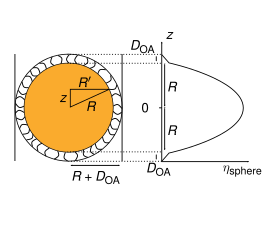
\includegraphics{looselyPackedNP_sphereProfile}
      \caption{\label{fig:looselyPackedNP:layerCharacterization:sphereProfile}Evaluation of the cross-section area fraction in comparison to a surrounding cylinder with respect to the height for a sphere with a core radius of $R$ and a oleic acid shell of thickness $D_\mathrm{surf.}$.}
    \end{figure}
    To model a nanosphere layer for the evaluation of the reflectivity of both SC-IOS-11 and SC-IOS-7, the area fraction of spheres in a layer needs to be formalized.
    The cross-sectional area with respect to an axis for a single sphere is given by a parabola, which is trivially derived using the Pythagorean theorem.
    For a sphere with a surfactant shell, \reffig{fig:looselyPackedNP:layerCharacterization:sphereProfile} can be used to determine the area fraction of the nanoparticle $\eta_\mathrm{part.}$ and the surfactant shell $\eta_\mathrm{surf.}$, which when evaluated with respect to a surrounding cylinder of radius $R_\mathrm{total} = R + D_\mathrm{surf.}$ are given by
    \begin{align}
      \eta_\mathrm{part.} (z)
        &\eq \begin{cases}
        \eta \frac{R^{2} - z^2}{R_\mathrm{total}^2}, &\mathrm{for\,}0<|z|<R, \\
        0,                                            &\mathrm{else},
        \end{cases}\\
      \eta_\mathrm{surf.} (z)
        &\eq \begin{cases}
          \eta \frac{R_\mathrm{total} - R^2}{R_\mathrm{total}^2}, &\mathrm{for\,}0<|z|<R, \\
          \eta \frac{R_\mathrm{total}^2 - z^2}{R_\mathrm{total}^2}, &\mathrm{for\,}R<|z|<R_\mathrm{total},\\
          0,                                            &\mathrm{else},
        \end{cases}
    \end{align}
    where $\eta$ is then the two-dimensional packing density of the surrounding cylinder in the layer.
    The scattering length density profile $\rho(z)$ of a layer of nanospheres is then given by
    \begin{align}
      \label{eq:looselyPackedNP:layerCharacterization:sldFromAreaFraction}
      \rho(z) \eq \rho_\mathrm{part.} \eta_\mathrm{part.}(z) + \rho_\mathrm{surf.} \eta_\mathrm{surf.}(z),
    \end{align}
    where $\rho_\mathrm{part.}$ and $\rho_\mathrm{shell}$ are the respective scattering length densities of the core and the shell.

    For a particle with a core-shell structure additionally to the surfactant shell the formulation can be extended.
    For simplicity, the particle size radius $R_\mathrm{part.} = R_\mathrm{core} + D_\mathrm{shell}$ and the total nanoparticle radius including the surfactant as $R_\mathrm{total} = R_\mathrm{core} + D_\mathrm{shell} + D_\mathrm{surf.}$ is defined and then the area fractions of the three components are given by
    \begin{align}
      \eta_\mathrm{core} (z)
        &\eq \begin{cases}
        \eta \frac{R_\mathrm{core}^{2} - z^2}{R_\mathrm{total}^2}, &\mathrm{for\,}0 < |z|<R_\mathrm{core}, \\
        0,                                               &\mathrm{else},
        \end{cases}\\
      \eta_\mathrm{shell} (z)
        &\eq \begin{cases}
          \eta \frac{R_\mathrm{part.}^2 - R_\mathrm{core}^2}{R_\mathrm{total}^2}, &\mathrm{for\,}0 < |z|<R_\mathrm{core}, \\
          \eta \frac{R_\mathrm{part.}^2 - z^2}{R_\mathrm{total}^2}, &\mathrm{for\,}R_\mathrm{core}<|z|<R_\mathrm{part.} \\
          0,                                            &\mathrm{else},
        \end{cases}\\
      \eta_\mathrm{surf.} (z)
        &\eq \begin{cases}
          \eta \frac{R_\mathrm{total}^2 - R_\mathrm{part.}^2}{R_\mathrm{total}^2}, &\mathrm{for\,}0<|z|<R_\mathrm{part.}, \\
          \eta \frac{R_\mathrm{total}^2 - z^2}{R_\mathrm{total}^2}, &\mathrm{for\,}R_\mathrm{part.} < |z| < R_\mathrm{total}, \\
          0,                                            &\mathrm{else}.
        \end{cases}
    \end{align}
    And the scattering length density profile is then given by
    \begin{align}
      \label{eq:looselyPackedNP:layerCharacterization:sldFromAreaFractionCoreShell}
        \rho(z) \eq& \rho_\mathrm{core} \eta_\mathrm{core}(z) + \rho_\mathrm{shell} \eta_\mathrm{shell}(z) + \rho_\mathrm{surf.} \eta_\mathrm{surf.}(z),
    \end{align}
    where $\rho_\mathrm{part.}$ and $\rho_\mathrm{shell}$ are the respective scattering length densities of the core and the shell.

    In this formulation it is nowstraight-forward to extend it to overlapping nanosphere layers by summing the respective area fractions $\eta_x$ for each layer before determining the SLD by \refeq{eq:looselyPackedNP:layerCharacterization:sldFromAreaFraction} or \refeq{eq:looselyPackedNP:layerCharacterization:sldFromAreaFractionCoreShell}.
    This procedure is performed for both SC-IOS-11 and SC-IOS-7, where as initial model a stack of nanospheres is given.
    Each layer is pitched on the vertical axis by $\sqrt{8/3} R_\mathrm{total}$, which is the vertical distance of two sphere centers for an ideal close sphere packing if $R_\mathrm{total}$ is the radius of a hard-sphere.
    The model is fitted by varying the two dimensional layer packing fraction $\eta$ and a shift from the initially assumed pitch $\Delta z$ for each layer respectively.

    The parameters for the nanosphere size, surfactant thickness and scattering length density are used as obtained from SAS, noting that the SLD are readjusted for the different X-ray wavelength at the reflectometer with respect
    to the small-angle scattering experiments.
    For SC-IOS-11, the core-shell structure obtained by SAXS and SANS on IOS-11 (\refsec{sec:looselyPackedNS:nanoparticle:sas}) is used for the nanospheres, and for SC-IOS-7 the single phase structure of IOS-7 is used.
    The particle size distribution is neglected in the formulation of the stack of nanoparticles as it is phenomenologically included in the fitted roughness of the layers.
    As roughness model a linearly increasing roughness $\sigma \eq \sigma_0 + \Delta \sigma z$ is used to describe a possibly increasing roughness with stack height.

  \paragraphNewLine{Polarized Neutron Reflectometry}
    Polarized neutron reflectometry has been performed on SuperADAM at the ILL for all discussed samples at a temperature of $300 \unit{K}$ and at a low temperature of $30 \unit{K}$.
    The distance between sample and detector for the experiments was $2.009 \unit{m}$ and a range of incident angles from $0 ^\circ \ldots 3 ^\circ$ is measured.
    The neutron wavelength was selected to $\lambda \eq 5.14 \unit{\angstrom}$ and $\lambda \eq 5.18 \unit{\angstrom}$ for the measurements at $300 \unit{K}$ and $30 \unit{K}$ respectively.
    The wavelength spread is in both cases $0.5 \%$ (FWHM) as provided by the instrumental scientists.
    The monochromator aperture is set to $1 \unit{mm}$ and the sample aperture to $0.5 \unit{mm}$ along the scattering direction for the measurements at $300 \unit{K}$, and to $3 \unit{mm}$ and $1 \unit{mm}$ for the measurements at $30 \unit{K}$.

    At room temperature, the samples are fixed by a vacuum suction and measured at a guide field of $4 \unit{mT}$, at a high magnetic field of $500 \unit{mT}$ and subsequently again at $4 \unit{mT}$ in remanence.
    For the measurements at $30 \unit{K}$, the samples are fixed in a cryostat using Apiezon vacuum grease and the guide field is measured to be $2.4 \unit{mT}$.
    The procedure is in each case to cool the samples from room temperature to $30 \unit{K}$ at guide field and measure the initial reflectivity.
    Then the reflectivity is measured at an applied field of $730 \unit{mT}$, and subsequently in remanence at guide field again.
    To study the reflectivity after field-cooling, the samples are heated above $200 \unit{K}$ and cooled back to $30 \unit{K}$ at an applied field of $730 \unit{mT}$.
    The reflectivity is then measured at the applied field and finally in remanence of the field-cooled state.

    For the room temperature measurements, a range of incident angles from $0^\circ \ldots 3 ^\circ$ is measured in $0.01 ^\circ$ steps with $20 \unit{s} - 60 \unit{s}$ counting time, with an linear increase with respect to the incident angle.
    In the $30 \unit{K}$ measurements, the range is increased to $4 ^\circ$ and the counting time is increased non-linearly in the range from $4 \unit{s} - 200 \unit{s}$ in accordance to the asymptotic behaviour of Fresnel's reflectivity, which drops in intensity with $q^4$.

    All measurements are performed with polarized neutrons, providing two reflectivity channels for each measurement, one for neutrons parallel to the magnetic field direction, and one for neutrons that are anti-parallel.
    For the layers prepared from IOS-11, an additional polarization analysis is performed for the low-temperature measurements to measure the spin-flip channel of neutrons coming from an anti-parallel incident state and are outgoing in a parallel state.
    For the remaining samples, no polarization analysis is performed.
    The polarization efficiency is measured from the direct beam to be $\approx 99 \%$ at guide field and high field.

    The detector images are scaled to it's respective monitor to correct for varying counting-times and fluctuating incident beam intensities.
    Due to a malfunction of the monitor for the field-cooled remanence measurement of 8BL-15-IOS-11, this specific measurement is scaled to the counting time instead.
    The detector images are reduced by integrating the detector dimension perpendicular to the scattering plane, providing a intensity map with respect to the incident angle and remaining detector dimension for each measurement and each channel.
    The coordinates are transformed to ($\alpha_i - \alpha_o$, $\alpha_i + \alpha_o$) using the pixel-splitting rebinning algorithm described in \refapp{ch:appendix:numericalMethods:rebinningPixelSplitting}.
    To obtain the reflectivity curves, a box in the range $\alpha_i - \alpha_o \eq -0.1 ^\circ \ldots 0.1 ^\circ$ is integrated, and the diffuse scattering is subtracted with the box integrals of the ranges $\alpha_i - \alpha_o \eq \pm (0.1 \ldots 0.2)$ in the intensity map.

    The same model as in XRR is used to describe the reflectivity of SC-IOS-11 and SC-IOS-7.
    The particle geometry and scattering length densities are used as obtained from SAS, and only the layer positions and packing densities are varied.

  \paragraphNewLine{Vibrating Sample Magnetometry}
    Pieces from the samples SC-IOS-11 and SC-IOS-7 are studied by vibrating sample magnetometry using a PPMS Evercool II (\refsec{ch:instruments:laboratoryInstruments:vsm}).
    Using a diamond cutter, $5 \times 5 \unit{mm^2}$ small pieces are cut and fixed on a Quartz sample holder using a low-temperature varnish (GE 7031).
    The samples are measured at $300 \unit{K}$ over a range of $\pm 9 \unit{T}$ with a sweeping rate of $5 \unit{mT \, s^{-1}}$.
    Furthermore, zero-field cooled and field cooled temperature-dependent magnetization measurements of the samples are performed by cooling the samples to $10 \unit{K}$ and measuring the magnetization while heating with a rate of $1.5 \unit{K \, min^{-1}}$.
    and at $30 \unit{K}$ over a range of $\pm 730 \unit{mT}$

    The magnetization data is rescaled in both cases, by performing a Langevin fit on the data obtained at $300 \unit{K}$.
    The obtained magnetic moment is used to determine the spontaneous magnetization $M_s$ of the by assuming the particle volume as it's obtained from SAXS as described in \refsec{ch:methods:vsm}.


\end{document}